\documentclass[11pt,a4paper]{article}

% --- Paquetes Principales ---
\usepackage[utf8]{inputenc}
\usepackage[T1]{fontenc}
\usepackage[spanish,es-tabla]{babel}
\usepackage[margin=2.5cm]{geometry}
\usepackage{graphicx}
\usepackage{booktabs}
\usepackage{caption}
\usepackage{microtype}
\usepackage{fancyhdr}
\usepackage{titlesec}
\usepackage{xcolor}
\usepackage{enumitem}
\usepackage{hyperref}

% --- Configuración de Enlaces y Colores ---
\definecolor{unsblue}{RGB}{27, 79, 114}
\definecolor{indiared}{RGB}{192, 57, 43}
\definecolor{darkslate}{RGB}{44, 62, 80}

\hypersetup{
    colorlinks=true,
    linkcolor=unsblue,
    citecolor=unsblue,
    urlcolor=unsblue
}

% --- Rutas de Figuras (Compilación desde raíz o desde carpeta latex/) ---
\graphicspath{{output/figures/}{../output/figures/}{figures/}}

% --- Formato de Títulos y Encabezados ---
\titleformat{\section}
  {\normalfont\Large\bfseries\color{unsblue}}{\thesection.}{0.8em}{}
\titleformat{\subsection}
  {\normalfont\large\bfseries\color{darkslate}}{\thesubsection.}{0.6em}{}

\pagestyle{fancy}
\fancyhf{}
\fancyhead[L]{\small\color{darkslate}Desarrollo Económico -- UNS}
\fancyhead[R]{\small\color{darkslate}Trabajo Práctico N° 1}
\fancyfoot[C]{\thepage}
\renewcommand{\headrulewidth}{0.4pt}

\setlength{\parskip}{0.6em}
\setlength{\parindent}{0pt}

% --- Datos de Portada / Encabezado ---
\title{\vspace{-1.5cm}\Large\textbf{Universidad Nacional del Sur}\\\large\textbf{Departamento de Economía}\\[0.4cm]
\huge\textbf{Trabajo Práctico N° 1: El Concepto de Desarrollo}\\[0.2cm]
\large Materia: Desarrollo Económico -- Licenciatura en Economía}
\author{\textbf{Estudiantes:} Mateo Barros y Grupo de Trabajo}
\date{Segundo Cuatrimestre -- 2026}

\begin{document}

\maketitle
\thispagestyle{fancy}
\vspace{-0.3cm}
\hrule
\vspace{0.6cm}

% ==============================================================================
% SECCIÓN 1: INTRODUCCIÓN AL PRÁCTICO Y DATOS
% ==============================================================================
El país que se nos adjudicó mediante sorteo fue \textbf{India}. Para poder establecer una comparación empírica y analizar las dimensiones del desarrollo, elegimos como país de referencia más desarrollado ---al menos en ciertos aspectos, no en todos--- a \textbf{Estados Unidos}.

A continuación, se presentan las comparaciones longitudinales de a pares para los tres indicadores seleccionados (\textit{PBI per cápita real}, \textit{Índice de felicidad} e \textit{Índice de Desarrollo Humano}) y, posteriormente, el análisis de la evolución simultánea de las tres dimensiones para el caso de India.

% ==============================================================================
% SECCIÓN 2: COMPARACIONES DE A PARES (INDIA VS. ESTADOS UNIDOS)
% ==============================================================================
\section{Comparaciones de a Pares: India vs. Estados Unidos}

\subsection{Producto Bruto Interno per Cápita (PBI pc)}

\begin{figure}[htbp]
    \centering
    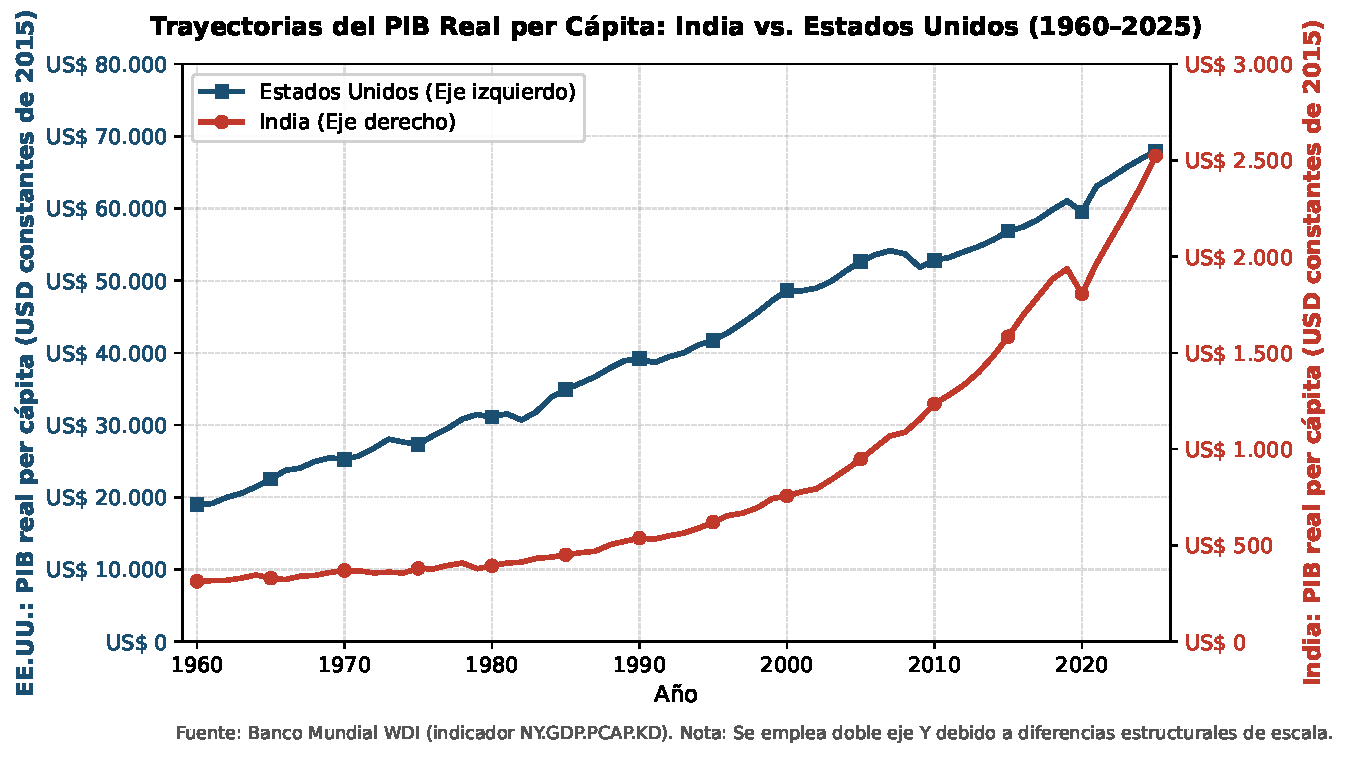
\includegraphics[width=0.92\textwidth]{02_gdp_india_vs_usa.pdf}
    \caption{Trayectorias del PIB Real per Cápita: India vs. Estados Unidos (1960--2025).}
    \label{fig:gdp_ind_usa}
\end{figure}

Cabe aclarar que las escalas de ambas curvas en la Figura \ref{fig:gdp_ind_usa} son distintas: el eje izquierdo corresponde a Estados Unidos (en miles de dólares) y el eje derecho, a India.

En el gráfico se observa una clara tendencia alcista en el PBI per cápita de India, explicada principalmente por la fuerte liberalización de su economía a comienzos de la década de 1990, junto con una serie de reformas estructurales que permitieron atraer inversión extranjera y abrir el país a nuevos mercados.

La amplia brecha entre los valores de PBI per cápita de India y de Estados Unidos puede explicarse, en parte, por la diferencia poblacional entre ambos países: hacia 2025, la población de India cuadruplicaba a la de Estados Unidos, lo que tiende a reducir el valor per cápita del indicador. Además, no debemos olvidar que estamos comparando a nuestro país con la economía de mayor PBI per cápita del mundo, por lo que esta diferencia resulta esperable.

Si bien este indicador no contempla una amplia variedad de variables ---como, por ejemplo, la distribución del ingreso entre los distintos segmentos productivos de la sociedad---, resulta útil porque permite dimensionar, de manera aproximada, la magnitud de la brecha de ingresos entre los habitantes de ambos países.

\newpage

\subsection{Índice de Felicidad (Satisfacción de Vida Autopercibida)}

\begin{figure}[htbp]
    \centering
    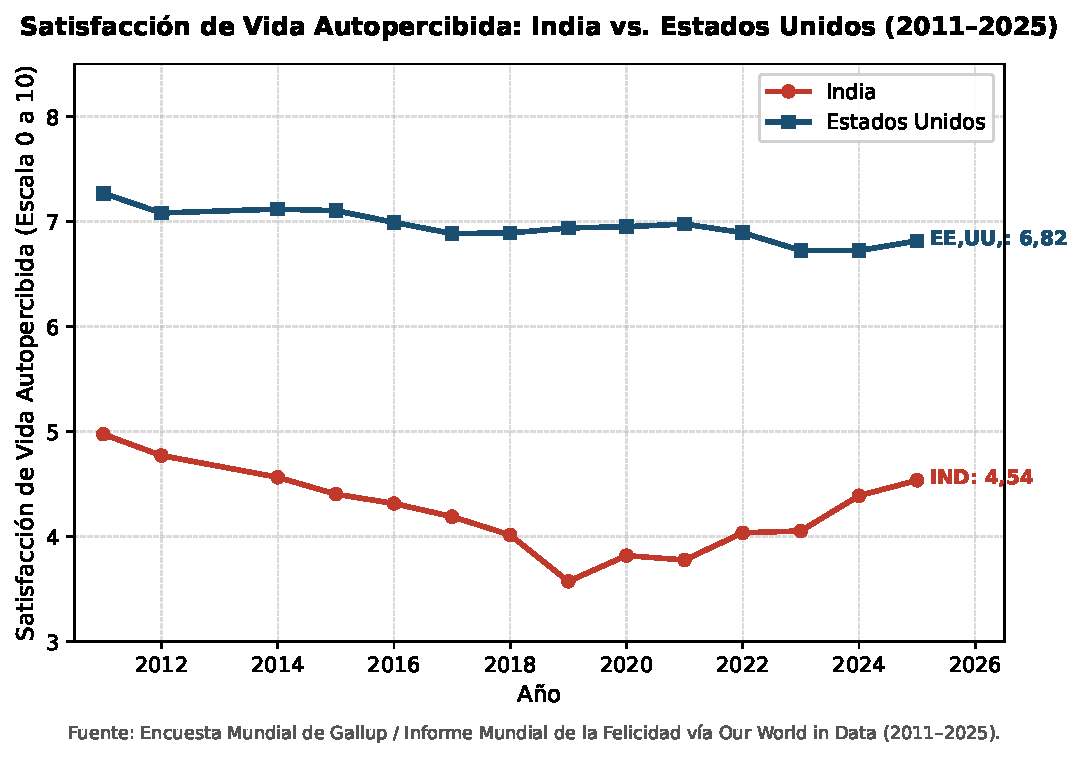
\includegraphics[width=0.92\textwidth]{03_happiness_india_vs_usa.pdf}
    \caption{Satisfacción de Vida Autopercibida: India vs. Estados Unidos (2011--2025).}
    \label{fig:happiness_ind_usa}
\end{figure}

A partir de este indicador (Figura \ref{fig:happiness_ind_usa}) observamos que India se mantiene consistentemente por debajo de Estados Unidos entre 2011 y 2025, con una diferencia marcada de alrededor de 2 puntos.

Cabe recordar que el índice de felicidad se construye a partir de varias variables explicativas, tales como el apoyo social, la expectativa de vida, la libertad para tomar decisiones, la generosidad y la percepción de la corrupción.

Profundizando en el gráfico, la caída de India entre 2011 y 2019 coincide con las fricciones generadas por reformas estructurales de shock: la desmonetización masiva de 2016, que golpeó fuertemente a la economía informal, y la implementación del GST (\textit{Goods and Services Tax}) en 2017. A esto se sumaron el incremento del desempleo juvenil urbano y el creciente estrés demográfico y medioambiental, factores que deterioraron el bienestar percibido pese a que el PBI agregado continuaba creciendo a tasas elevadas.

Entre 2018 y 2020, período en el que transcurrió la pandemia de Covid-19, se observan los niveles más bajos de la serie, en torno a 3,8 puntos, explicados por las restricciones y el confinamiento vigentes durante esos años.

La recuperación post pandemia se refleja en una suba de aproximadamente 1 punto, impulsada por la consolidación de la seguridad digital y financiera, y por el incremento de la inversión estatal en infraestructura y logística.

\newpage

\subsection{Índice de Desarrollo Humano (IDH)}

\begin{figure}[htbp]
    \centering
    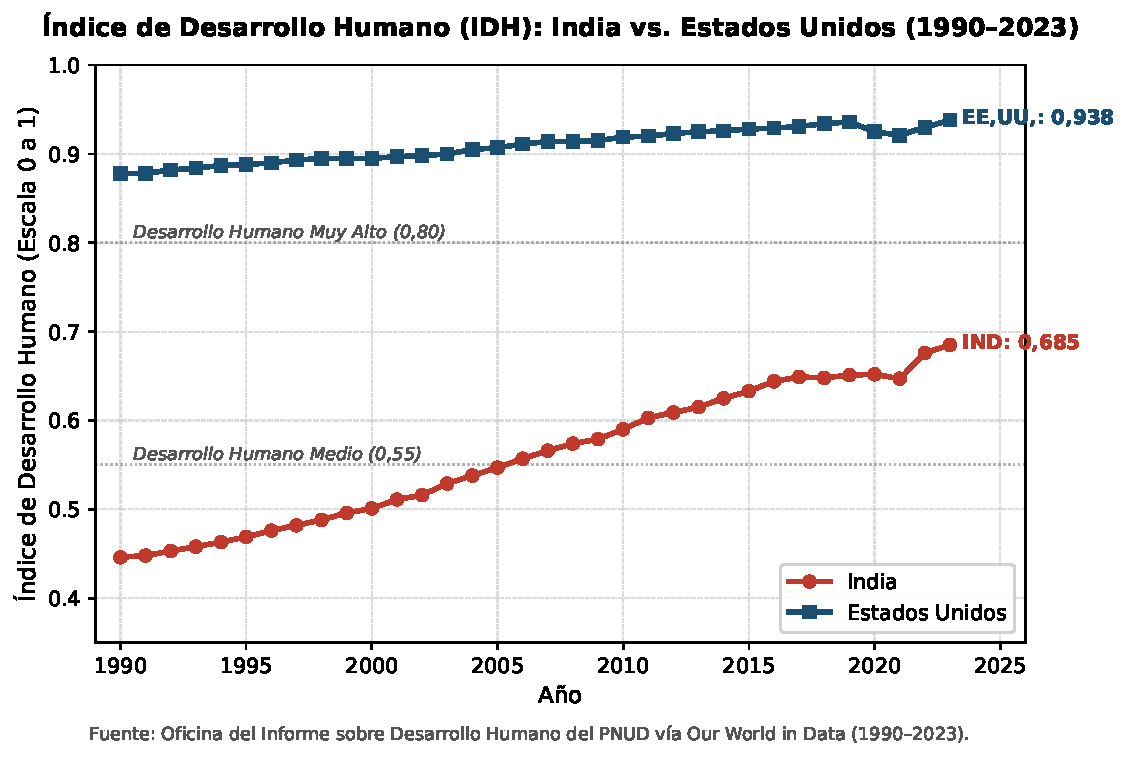
\includegraphics[width=0.92\textwidth]{01_hdi_india_vs_usa.pdf}
    \caption{Índice de Desarrollo Humano (IDH): India vs. Estados Unidos (1990--2023).}
    \label{fig:hdi_ind_usa}
\end{figure}

Finalizamos con otro indicador ampliamente utilizado: el Índice de Desarrollo Humano (Figura \ref{fig:hdi_ind_usa}), el cual sintetiza logros en salud (expectativa de vida), educación (años promedio y esperados de escolaridad) e ingreso per cápita.

La trayectoria de India muestra una tendencia claramente alcista, consolidando un avance sostenido en su desarrollo humano gracias al crecimiento del PBI per cápita, al aumento de la expectativa de vida y a la mayor escolarización de su población. Aun así, se evidencia una brecha considerable frente a un país de desarrollo consolidado como Estados Unidos.

\subsection{Balance de las Comparaciones Internacionales}

Una vez observados los tres índices para ambos países, podemos arribar a una serie de conclusiones sobre las comparaciones:

\begin{itemize}[leftmargin=1.5em]
    \item \textbf{Heterogeneidad de brechas:} Las tres comparaciones muestran una brecha de desarrollo persistente entre India y Estados Unidos, aunque de magnitud y dinámica distinta según el indicador. En términos de PBI per cápita, la diferencia es la más pronunciada de las tres, condicionada tanto por el tamaño poblacional de India como por el punto de partida de cada economía; sin embargo, es también donde se observa la convergencia más marcada en los últimos años, impulsada por la apertura comercial y financiera iniciada en los noventa.
    \item \textbf{Rigidez del bienestar subjetivo:} El índice de felicidad, en cambio, exhibe una brecha más estable a lo largo del tiempo: al depender de factores como el apoyo social, la confianza institucional y la percepción de corrupción ---y no solo del ingreso---, no acompaña al mismo ritmo las mejoras económicas, e incluso se vio afectado por shocks propios de la transición estructural india y por la pandemia.
    \item \textbf{Convergencia acumulativa en capacidades:} El IDH, por su parte, presenta una convergencia más gradual y sostenida, reflejo de las mejoras acumuladas en salud y educación.
\end{itemize}

En conjunto, estas comparaciones sugieren que el crecimiento económico es una \textbf{condición necesaria pero no suficiente} para el desarrollo: reduce algunas brechas materiales de manera relativamente rápida, pero las dimensiones vinculadas al bienestar subjetivo y a las capacidades humanas convergen de forma más lenta y desigual.

\newpage

% ==============================================================================
% SECCIÓN 3: ANÁLISIS SIMULTÁNEO PARA INDIA
% ==============================================================================
\section{Análisis Simultáneo de Indicadores para India}

Para finalizar el trabajo, analizamos a India de manera aislada, integrando la evolución de los tres índices. 

Dado que no es posible representar tres series con escalas tan distintas en un único gráfico con más de dos ejes sin comprometer la legibilidad, optamos por presentar la información en dos gráficos complementarios: uno dedicado a la trayectoria del bienestar subjetivo (Figura \ref{fig:happiness_ind}) y otro que combina el PBI per cápita con el IDH en doble eje temporal extendido (Figura \ref{fig:hdi_gdp_ind}).

\begin{figure}[htbp]
    \centering
    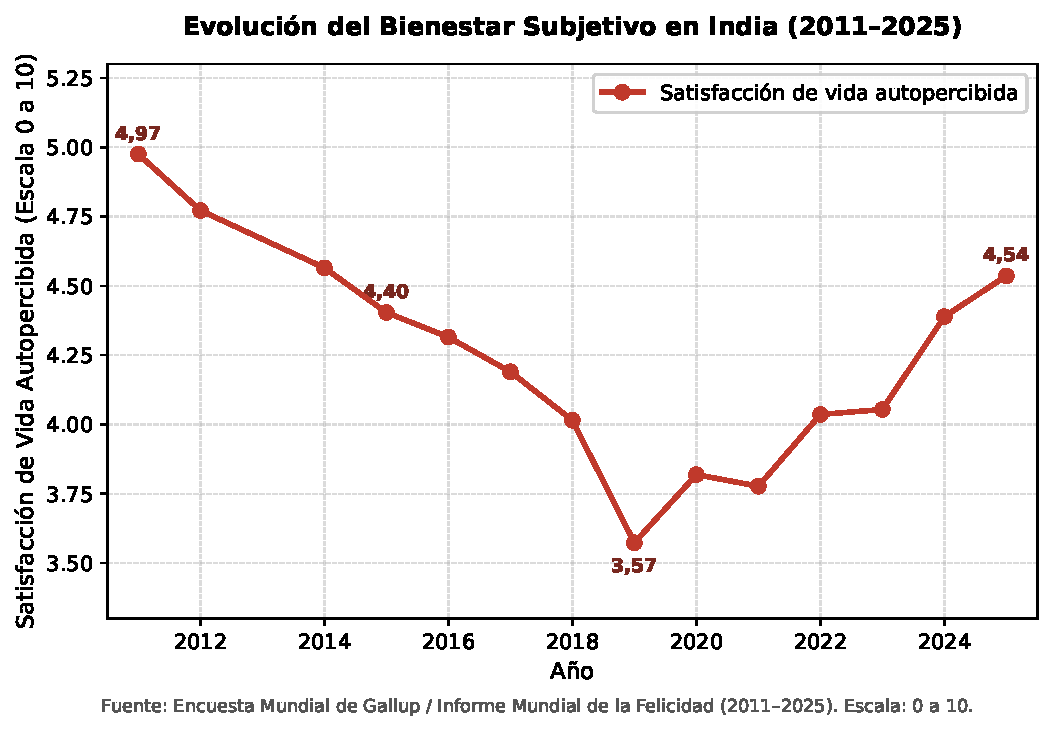
\includegraphics[width=0.88\textwidth]{04_happiness_india.pdf}
    \caption{Evolución del Bienestar Subjetivo en India (2011--2025).}
    \label{fig:happiness_ind}
\end{figure}

En cuanto al índice de felicidad (Figura \ref{fig:happiness_ind}), observamos que su trayectoria no acompaña la tendencia alcista sostenida del PBI per cápita ni del IDH: cae de manera marcada entre 2011 y 2019 ---en coincidencia con las reformas de shock antes mencionadas--- y recién comienza a recuperarse después de la pandemia, sin llegar a alcanzar los niveles iniciales de la serie. Esto evidencia que, para India, el crecimiento económico y la mejora en salud y educación no se tradujeron de manera directa en una mayor percepción de bienestar.

\newpage

\begin{figure}[htbp]
    \centering
    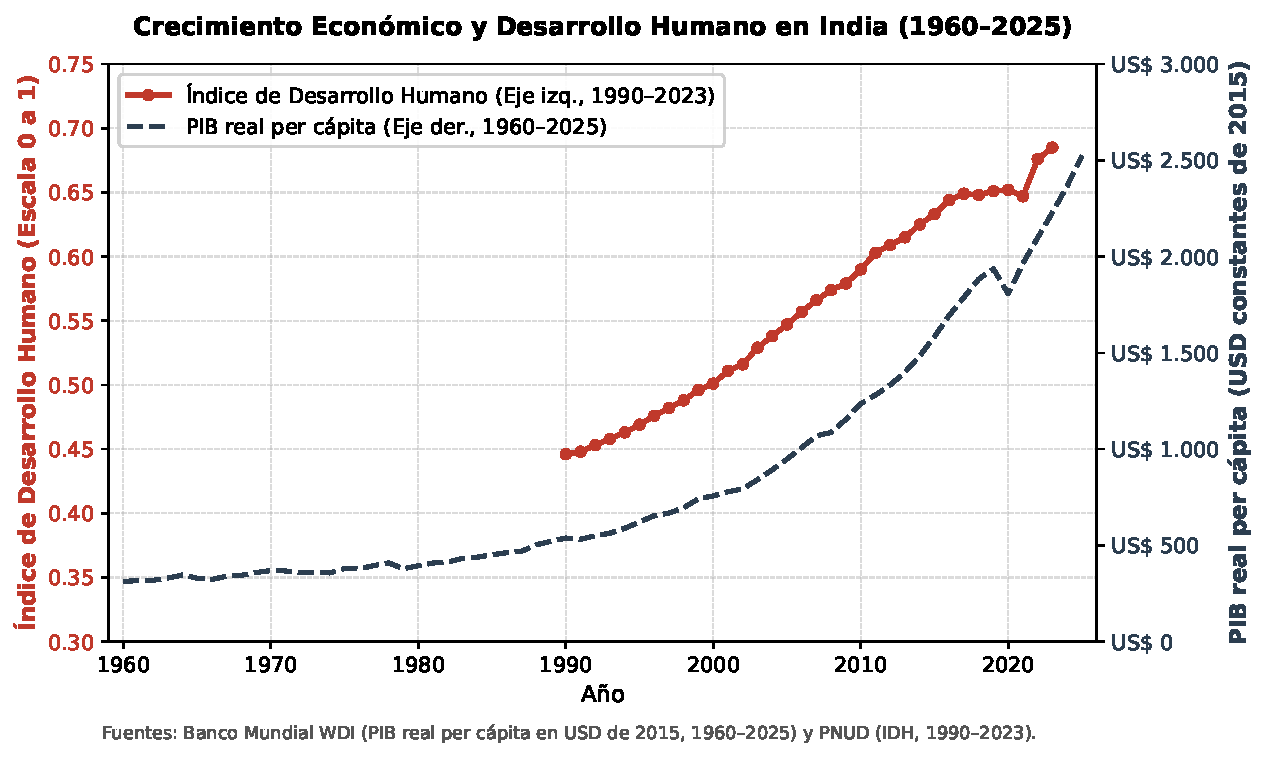
\includegraphics[width=0.92\textwidth]{05_hdi_and_gdp_india.pdf}
    \caption{Crecimiento Económico y Desarrollo Humano en India (1960--2025).}
    \label{fig:hdi_gdp_ind}
\end{figure}

Al analizar conjuntamente la evolución del Índice de Desarrollo Humano (IDH) y del PBI real per cápita para India a lo largo del período 1960--2025 (Figura \ref{fig:hdi_gdp_ind}), se observan patrones estructurales diferenciados:

\begin{enumerate}[leftmargin=1.5em]
    \item \textbf{Etapa de estancamiento inicial (1960--1990):} Durante las tres primeras décadas, el ingreso por habitante registró un dinamismo sumamente modesto, pasando de US\$ 312,78 a US\$ 537,87 constantes (a una tasa promedio anual cercana al $1,8\%$), en un contexto dominado por un esquema de economía cerrada y fuerte regulación estatal (\textit{License Raj}).
    \item \textbf{Aceleración y co-movimiento post-1990:} A partir de la década de 1990, tras la liberalización económica y la integración a los mercados globales, ambas series quiebran su tendencia previa. El PBI per cápita real se expande de manera acelerada, multiplicándose por casi 5 veces hasta alcanzar US\$ 2.523,44 constantes en 2025 (superando los US\$ 10.000 en términos de paridad de poder adquisitivo). En paralelo, el IDH experimenta un salto del $+53,6\%$, aumentando de 0,446 en 1990 a 0,685 en 2023. Esta evolución permitió a India abandonar la categoría de \textit{Desarrollo Humano Bajo} y consolidarse en el rango de \textit{Desarrollo Humano Medio}.
    \item \textbf{Interpretación teórica y límites del crecimiento:} Los datos reflejan la retroalimentación virtuosa entre crecimiento del ingreso monetario y expansión de capacidades humanas (salud y educación, en línea con el enfoque de Amartya Sen). El incremento del producto amplió la base material y los recursos fiscales para expandir la cobertura sanitaria y la escolarización. No obstante, en los años más recientes se evidencia un desacople de pendientes: mientras el PBI per cápita mantiene un crecimiento exponencial, el IDH tiende a moderar su avance.
\end{enumerate}

Integrando ahora el índice de felicidad a este análisis conjunto, la correlación entre los tres indicadores resulta débil: mientras que el PBI per cápita y el IDH muestran una asociación positiva razonable ---ambos crecen de forma sostenida, aunque a ritmos distintos---, la felicidad se mueve de manera prácticamente independiente, e incluso en sentido contrario durante buena parte del período analizado.

Esto tiene sentido si consideramos que el PBI y el IDH capturan dimensiones más objetivas y acumulativas del desarrollo (ingreso, salud, educación), mientras que la felicidad depende en gran medida de factores coyunturales y subjetivos ---estabilidad institucional, empleo de calidad, percepción de corrupción--- que no necesariamente mejoran al mismo ritmo que la economía.

A partir de este análisis concluimos que el crecimiento económico no implica necesariamente desarrollo, y que el desarrollo, a su vez, no implica necesariamente bienestar percibido: la apertura económica de India es un proceso relativamente reciente, y los cambios estructurales necesarios para traducir ese crecimiento en desarrollo pleno ---y en una mejora del bienestar subjetivo de la población--- todavía están en curso. La pregunta que queda abierta es si, en los próximos años, esa brecha entre crecimiento, desarrollo y bienestar logrará cerrarse.

\end{document}
